
\begin{enumerate}
		\item Дата собрания 3.10.14
		\item Цель:
		\begin{itemize}
			\item Укрепить конструкцию робота
			\item Разнести колеса по углам конструкции для увеличения площади колесной базы
			\item Закрепить основные узлы управления робота на конструкции с максимально легким доступом к ним
			\item Оптимизировать программу, перенести управление передвижением робота с кнопок на джойстик
		\end{itemize}
		\item Результаты:
		\begin{itemize}
			\item Конструкция робота была укреплена, центр тяжести снижен 
			\item Двигатели были закреплены по углам конструкции, одновременно закрепляя ее
			\item На осях был закреплен второй ряд колес определенным образом для лучшего управления(Рисунок 2,3)
		\end{itemize}
		\begin{figure} [h]
			\centering
			\begin{minipage}{0.3\linewidth}
				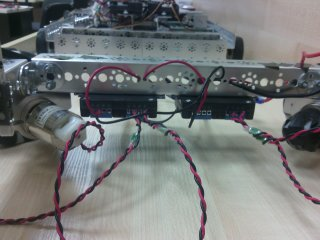
\includegraphics[width=35mm,height=35mm]{3_1_robot}\\ Рисунок 3
			\end{minipage}
			\begin{minipage}{0.3\linewidth}
				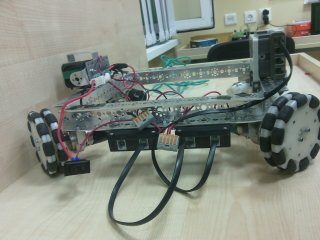
\includegraphics[width=35mm,height=35mm]{3_2_robot}\\ Рисунок 4
			\end{minipage}
			\begin{minipage}{0.3\linewidth}
				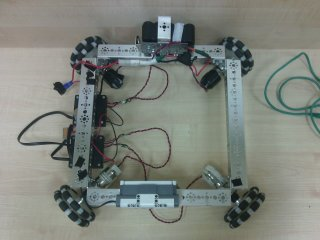
\includegraphics[width=35mm,height=35mm]{3_3_robot}\\ Рисунок 5
			\end{minipage}
		\end{figure}
		\item Идеи и планы для следующего занятия:
		\begin{itemize}
			\item Начать строить механизм захвата и подъема шариков. В качесте механизма подъема можно использовать ножничный подъемник, механизм захвата еще обдумывается
		\end{itemize}
	\end{enumerate}
\newpage